\section{Experiments}\label{sec:experiments}
15 kinds of optimizations choices for AES are explored in our experiments. The synthesis results of these implementations vary in architectures as well as in resource consuming and time cost. We synthesized these RTL descriptions in Synopsys using TSMC $0.18um$ standard cell library. Table \ref{xxxx} shows the main measuring dimensions of these circuits. We could see that, configuration with the most modules has 2.5 times of gates number of that with fewest modules and 20\% of the cycles. Thus, the reconfigurations do make sense, since users can get considerable trade-offs between space and time. Table \ref{table:com} is about the comparison with other implementations. Ours provide many kinds of configurations which have different gates, and have high frequency.
%%%%%%%%%%%%%%%%%%%%%%%%%%%%%%%%%%%%%%%%%%%%%%%%%%%%%%%%%%%%%%%%%%%%%%%%%
\begin{table}[h]
\centering
\caption{Area and Time cost of AES}
\begin{tabular}{|r|rr||r|rr|} \hline
\textit{conf.} & Gates & Cycles & \textit{conf.} & Gates & Cycles\\ \hline
\textit{(1,1)} & 6004 & 218 & \textit{(4,4)} & 7828 & 71 \\
\textit{(1,2)} & 6314 & 200 & \textit{(8,1)} & 8599 & 78 \\
\textit{(1,4)} & 6824 & 191 & \textit{(8,2)} & 8875 & 60 \\
\textit{(2,1)} & 6398 & 138 & \textit{(8,4)} & 9315 & 51 \\
\textit{(2,2)} & 6742 & 120 & \textit{(16,1)} & 11310 & 63 \\
\textit{(2,4)} & 7164 & 111 & \textit{(16,2)} & 11686 & 50 \\
\textit{(4,1)} & 7057 & 98 & \textit{(16,4)} &12069 & 41 \\ \cline{4-6}
\textit{(4,2)} & 7350 & 80 & \multicolumn{3}{c|}{} \\ \hline
\end{tabular}
\label{xxxx}
\end{table}
%%%%%%%%%%%%%%%%%%%%%%%%%%%%%%%%%%%%%%%%%
%\begin{table}[h]
%\centering
%\caption{Area and time cost of AES}
%\subtable[Cycles]{
%\begin{tabular}{|r|rrr|}\hline
% & \textit{1} & \textit{2} &  \textit{4} \\ \hline
%\textit{1} & 218 & 200 & 191 \\
%\textit{2} & 138 & 120 & 111 \\
%\textit{4} & 98 & 80  & 71 \\
%\textit{8} & 78 & 60  & 51\\
%\textit{16}& 63 & 50  & 41 \\ \hline
%\end{tabular}
%}
%\subtable[Gates]{
%\begin{tabular}{|r|rrr|}\hline
% & \textit{1} & \textit{2} &  \textit{4} \\ \hline
% \textit{1}  & 6004 & 6314 & 6824 \\
% \textit{2}  & 6398 & 6742 & 7164 \\
% \textit{4}  & 7057 & 7350 & 7828 \\
% \textit{8}  & 8599 & 8875 & 9315 \\
%\textit{16} & 11310& 11686 & 12069 \\ \hline
%\end{tabular}
%}
%\label{xxxx}
%\end{table}
\begin{table}[h]
\centering
\caption{Comparison with other AESs}
\begin{tabular}{|l|r|r|r|c|}\hline
Work & Tech & Gates & Freq & Conf \\ \hline
\cite{Akashi:AES} & $0.18um$ & 7226 & $138_{MHz}$ &  \\ \cline{1-4}
\cite{Martin:AES} & $0.35um$ & 3595 & $100_{KHz}$ & 1\\ \cline{1-4}
%[6] & $0.25um$ & 12000 & $100_M$ & 1 \\ \cline{1-4}
\cite{Norbert:AES} & $0.6um$ & 8541 & $50_{MHz}$ & \\ \hline
\cite{Yibo:AES} & $0.18um$ & 6986 & $180_{MHz}$ & 3 \\ \hline
Ours & $0.18um$ & 6004,...,12069 & $180_{MHz}$ & 15 \\ \hline
\end{tabular}
\label{table:com}
\end{table}
For silicon technology the area-time tradeoff has been nicely formalized by theorists as ``AT'' (area and time) bounds. Author in paper\cite{AT} shows that:
\begin{equation}
AT^n = constant, \;\;\;n\; is\; between\; 1\; and\; 2
\label{eq:at}
\end{equation}
Figure\ref{fig-mesure} is the two-dimension diagram between area-time of our AES implementations. The blue line is about gates and cycles of each implementation. And green line is function $xy=750000$. It reveals the area-time bounds approximately in keeping with \eqref{eq:at}, when $n=1$ and $constant = 750000$.
\begin{figure}[thbp]
\centering
\epsfig{file=mesure4.eps,width=0.7\columnwidth}
\caption{Configurations and Resource cost of AES}
\label{fig-mesure}
\end{figure}
\subsection{Sythesis result of SCM, DCT and FFT}
%In example SCM, there is a $fold$ re-configurable construct with 4 variables, so totally it has 3 different %configurations. FFT has 3 $forloop$. Since each $forloop$ provides 3 optimization choices, FFT has as many as 27 %kinds of configurations. DCT has also 3 $forloop$ and 36 kinds of implementations (Implementations of these %three algorithm are in Appendix B).
Table \ref{table:confs} shows area and time cost of some configurations of these three algorithms.
%\vspace{-3ex}
\begin{table}[hb]
\centering
\caption{Some Confs. of SCM, FFT and DCT}
\begin{tabular}{|r|rr|r|rr|} \hline
\multicolumn{3}{|c|}{SCM} & \multicolumn{3}{c|}{DCT} \\ \hline
%DFT & & & FFT & & \\ \hline
\textit{conf.} & Gates & Cycles & \textit{conf.} & Gates & Cycles \\ \hline
\textit{(1)} & 1621 & 9 & \textit{(1,1,1)} & 4562 & 17 \\
\textit{(2)} & 2782 & 5 & \textit{(1,1,2)} & 4903 & 13 \\
\textit{(4)} & 4738 & 3 & \textit{(1,1,4)} & 5104 & 11 \\ \cline{1-3}
\multicolumn{3}{|c|}{FFT} & \textit{(1,1,8)} & 5208 & 10 \\ \cline{1-3}
\textit{conf.} & Gates & Cycles & \textit{(1,2,1)} & 4711 & 15 \\ \cline{1-3}
\textit{(1,1,1)} & 4562 & 13 & \textit{(1,2,8)} & 4806 & 14 \\
\textit{(1,1,2)} & 4923 & 11 & \textit{(1,4,1)} & 5298 & 8 \\
\textit{(1,1,4)} & 5133 & 10 & \textit{(1,4,8)} & 5362 & 7 \\
\textit{(1,2,4)} & 5427 & 8 & \textit{(2,4,8)} & 5503 & 5 \\
\textit{(1,4,4)} & 5540 & 7 & \textit{(4,4,8)} & 5642 & 4 \\
\textit{(2,1,1)} & 5761 & 5 & \textit{(2,4,4)} & 5419 & 6 \\
\textit{(4,4,4)} & 5902 & 4 & \textit{(1,2,4)} & 5179 & 9 \\ \hline
\end{tabular}
\label{table:confs}
\end{table}
Column $conf.$ is the serial number of configurations. Gates is the number of gate, Cycles is the number of cycle. They are all synthesized under frequency $180_{MHz}$.
%%%%%%%%%%%%%%%%%%%%%%%%%%%%%%%%%%%%%%%%%%
